%\chapter{T-Ringの設計実装}
\chapter{設計と実装}
\begin{large}
\begin{quote}
%本章では,T-Ringにおける詳細な設計,実装について解説する.
本章では,本システムにおける機能要件,
概要,設計,さらに実装について説明する.
\end{quote}
\end{large}
\clearpage


\section{設計}

\subsection{機能要件}\label{sec:requirements}
ここでは本システムの設計にあたって,
\ref{sec:objective}で述べた本研究の目的を
達成するために必要となる機能について言及する.
%ここでは,\ref{sec:problems}で述べた既存研究における問題点を
%解決するという目的を達成するために必要となる機能について言及する.

\begin{enumerate}
\item{リアルタイム性}\\
時間的制約を伴ったタスクの処理が必要なアプリケーションを想定した場合,
オペレーティングシステムとして
リアルタイム処理を行えるものを選択すべきであり,
無線センサネットワークを用いた環境モニタリングでは,
%モニタリング対象の行動に変化があった際には,
イベント発生に応じてタスクを優先度を変化させる必要がある.
%このような時間的制約を伴ったタスクの処理が必要なアプリケーションを想定した場合,
%オペレーティングシステムとして
%リアルタイム処理を行うことが可能なものを選択することが多い.
また,ターゲットトラッキングにおいても同様に,
対象の検知は適時にゲートウェイまで届けられなければならない.
%イベントを検知したセンサの周辺ノードはそのイベントを監視し,
%ラップトップやベースステーションのような外界と通信する機能を持った
%シンクノードに対してイベントの発生を知らせるのだが,
%ターゲットトラッキングにおいて,
%対象を検知し,その旨をシステムのゲートウェイノードに警告するタスクにより
%中継されたデータは,
%適時にゲートウェイまで届けられるべきである.
%したがって,環境モニタリングと同様に
%ターゲットトラッキングでもリアルタイムオペレーティングシステムを採用すべきである.
\newline
%\item{省資源性かつ低オーバヘッド}\\
\item{低消費電力}\\
森林火災検知システムにおけるネットワークライフタイムは,
火災シーズンを上回ることが望ましく,
%一般的にそれぞれのノードが数週間に渡って稼働することは難しいのが現状である.
%したがってこの要件を満たすためにも,
%エネルギーの消費を抑えるようなシステムを提案する必要がある.
野生動物の生態調査を行う際にも,
%調査対象の特徴によっては,
現地調査を複数回行うことが困難となる場合もあるため,
資源の限られたセンサノードにおいて低オーバヘッドを
維持することは極めて重要である.
%無線センサネットワークに用いられる小型デバイスにおける
%バッテリの駆動時間は,一般的なラップトップなどと比較して
%かなり短いのが現状である.
%バッテリを交換する回数が増えるにつれ,
%無線センサネットワークから得られる利益は減少してしまうことから,
%火災検知システムと同様に,省エネルギーが実現できるような
%システム構成が求められている.
監視システムアプリケーションを用いた任務でも,
%数日から数ヶ月にかけて行われるものが一般的であり,
%任務中の秘密保持の重大性や
%任務が敵の管轄地域行われる場合もあることから,
%近づきにくさ
任務期間中に資源の制限されたセンサデバイスの手動による充電はできないことがほとんどであることから,
同様の機能が必要であることが考えられる.
%したがって任務期間中継続して使用するために,
%監視システムにおけるアプリケーションでは
%センサデバイスの寿命を向上させるような
%省エネルギーな構成が必要とされる.
\end{enumerate}



\subsection{システム概要}
%本研究では,Contikiにスケジューラを実装することで,
%省資源性かつ低オーバヘッドを実現する.
前述のとおり,Contiki\cite{Dunkels:2004:CLF:1032658.1034117}
はイベントモデルであるため,
%省資源でありつつ,オーバヘッドを
電力消費を低く維持することが可能である.
%またContikiにおけるProtothreads\cite{Dunkels:2006:PSE:1182807.1182811}は,
%マルチスレッド型のオペレーティングシステムのようにプログラムを記述できるため,
%イベントモデルの欠点であるプログラムの書き辛さを改善することができ,
%Protothreadsとスレッドモデルのオペレーティングシステムは関係が密であると推測できる.
%したがって,今回のアプローチとして,Protothreadsを採用する.
また\ref{sec:change_tasks}で示したように,
一般的なスレッドモデルではレジスタの状態を保存しておくことにより
タスクの切り替えを実現していることに対して,
ContikiにおけるProtothreads\cite{Dunkels:2006:PSE:1182807.1182811}は,
戻り値を利用することでタスクのCPUの利用を放棄しつつ,
一貫性を保つことが可能であるため,
他のスレッドモデルのオペレーティングシステムと比べて,
エネルギーの消費を軽減できる設計となっている.
しかしながら,Protothreadsを使用した場合,
タスクの実行を中断させるプリエンプションができないため,
本システムでは適時処理が必要なイベントが発生した際には,
コンテキストを保存し,スレッドを切り替えることができるような
設計が必要となる.

本システムの全体像を図\ref{fig:system_overview}に示す.
本システムは,ひとつのイベントループと多数のイベントハンドラから構成される.
イベントループはイベントの到着を待ち,
イベントが届くとイベントに関連付けられているイベントハンドラを実行する.
しかしながら,通常のイベントモデルのオペレーティングシステムと異なり,
本システムではリアルタイム処理の必要なイベントが発生する場合を想定している.
イベントループ実行中に,リアルタイムイベントが発生した場合には,
現在実行中のタスクをプリエンプションし,
スレッドを切り替え,リアルタイムタスク実行後再びイベントループの実行を再開する.
%スレッドモデルは図\ref{fig:threads_model}に示されるように,
%複数のスレッドから構成され,
%各スレッドはそれぞれ独立に実行ストリームを持っており,
%低い優先度のスレッドは高い優先度のスレッドにプリエンプションされるという特徴を持つ.
また,本システムではリアルタイムタスク実行中における
多重割り込みはしないものとする.





%イベントモデルではイベント駆動型プログラミングによってアプリケーションが記述される.
%イベントハンドラは寿命の短いrun-to-completionで記述され,
%プリエンプションされることがない.
%つまり,イベントモデルはタスクは関数呼び出しと等価であり,
%実行ストリームがひとつで実現されるため各タスクでローカル変数の領域を共有可能であることから,
%省資源かつ低オーバヘッドで並列性を実現できる.





%イベントモデルで構築されたオペレーティングシステムは全てのタスクをイベントによって起動し,
%run-to-completion で実行する形態のオペレーティングシステムである.
%イベントモデルは図\ref{fig:event_model}に示されるように,
%ひとつのイベントループと多数のイベントハンドラから構成される.
%イベントループはイベントの到着を待ち,
%イベントが届くとイベントに関連付けられているイベントハンドラを実行する.
%イベントモデルではイベント駆動型プログラミングによってアプリケーションが記述される.
%イベントハンドラは寿命の短いrun-to-completionで記述され,
%プリエンプションされることがない.
%つまり,イベントモデルはタスクは関数呼び出しと等価であり,
%実行ストリームがひとつで実現されるため各タスクでローカル変数の領域を共有可能であることから,
%省資源かつ低オーバヘッドで並列性を実現できる.
%また,各タスクが不可分に実行されるので共有資源に対する排他制御が不要となり,
%安全性が高い.
%さらに,CPU の特殊な機能を用いなくても実装できるので移植性も高い.
%本節では,TinyOSとContikiをイベントモデルの例として提示し,
%それぞれの特徴について言及する.


%スレッドモデルは図\ref{fig:threads_model}に示されるように,
%複数のスレッドから構成され,
%各スレッドはそれぞれ独立に実行ストリームを持っており,
%低い優先度のスレッドは高い優先度のスレッドにプリエンプションされるという特徴を持つ.
%スレッドモデルではユーザはあたかもCPUを占有しているかのように
%一連の処理をひとつのスレッドとして記述することができるため,
%プログラムが書きやすい.
%また,プリエンプションを行うことも想定しているため,
%%ジョブの実行を設定された時間通りに作動させる,
%ハードリアルタイム処理をサポートすることができる.





\begin{figure}[htbp]
 \begin{center}
  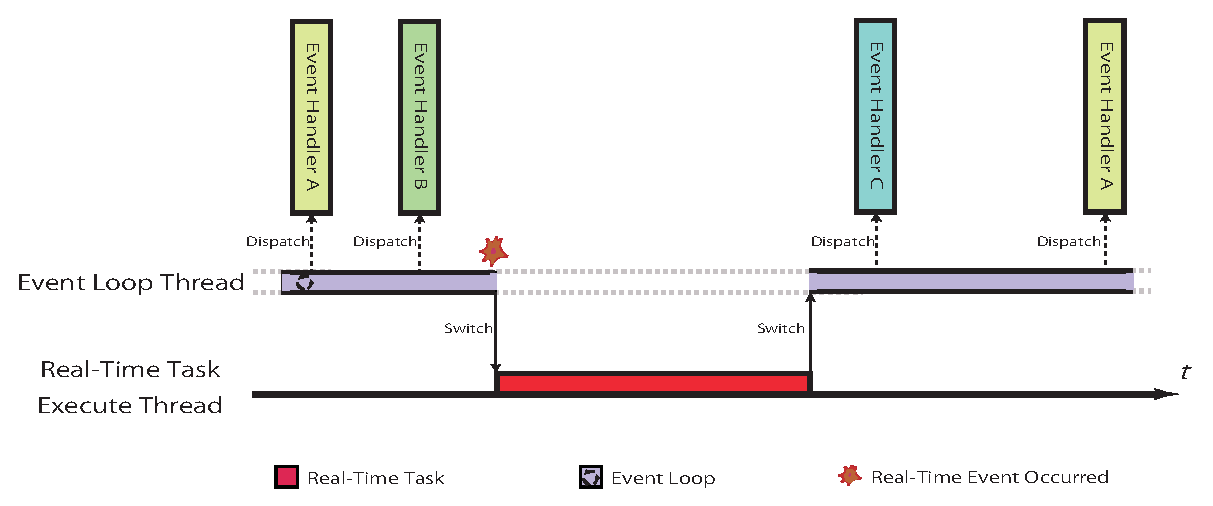
\includegraphics[width=150mm]{./images/system_overview.eps}
 \end{center}
 \caption{システム概要}
 \label{fig:system_overview}
\end{figure}


\subsection{システム構成}
%本節では,T-Ringシステムの設計について述べる.T-Ringを構成する保存ピアはネットワークモジュール,センサ情報管理モジュール,データ保存モジュール,データ取得モジュール,保存ピア発見モジュール,センサ管理モジュール,アプリケーションモジュールの7つのモジュールによって構成される.図\ref{fig:sysconf}がシステム構成図であり,各モジュール間でのデータの受け渡しが記述されている.
本節では,本システムのアーキテクチャ(図\ref{fig:system_architecture})を示し,
各モジュールについて詳しく説明する.


\begin{figure}[htbp]
 \begin{center}
  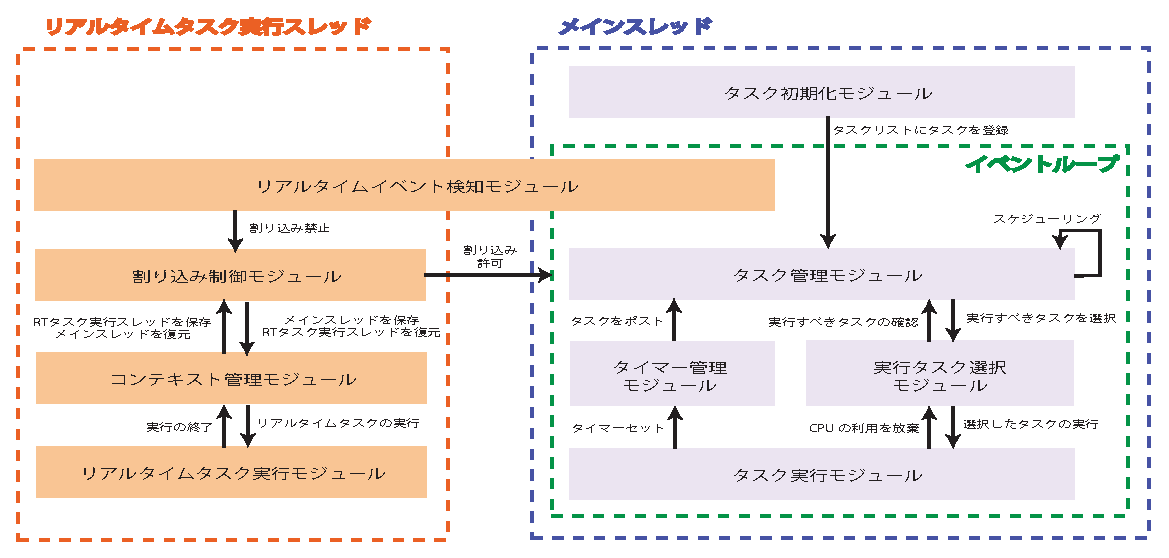
\includegraphics[width=150mm]{./images/system_architecture.eps}
 \end{center}
 \caption{システムアーキテクチャ}
 \label{fig:system_architecture}
\end{figure}


\subsubsection{タスク初期化モジュール}

\vspace{0.5em}タスク初期化モジュールは,アプリケーション開発者によって
初期化されたタスクをカーネルが保持するタスクリストに登録する.
リアルタイムタスクを初期化する際には,
そのタスクのコンテキストを保存するためのスタックも
同時に初期化しておく.
本モジュールはアプリケーションがデプロイされたときにのみ実行され,
イベントループ内で実行されるモジュールと異なり,
複数回実行されることはない.



\subsubsection{タスク管理モジュール}

\vspace{0.5em}ここではタスク初期化モジュールにて,
登録されたタスクをタスクリストに登録し,
スケジューリングアルゴリズムに従って,
タイマー管理モジュールによってポストされるタスクを
実行される順番に並び替える.
実行タスク選択モジュールからの問い合わせがあった際には,
スケジューリング後の最も優先度の高いタスクのアドレスを渡す.



\subsubsection{実行タスク選択モジュール}

\vspace{0.5em}タスク実行モジュールにおいて,
実行中のタスクがCPUの利用を放棄した場合,
実行タスク選択モジュールにて,
次に実行するタスクを選択するために,
タスク管理モジュールに実行が最優先とされるタスクについて尋ねる.
タスク管理モジュールからの応答を待ち,
受け取ったタスクを次に実行するべく,
タスク実行モジュールへと引き渡す.



\subsubsection{タスク実行モジュール}

\vspace{0.5em}タスク実行モジュールでは,
タスク選択モジュールにて選択されたタスクを実行する.
実行中のタスクがCPUの利用を放棄した場合には,
次に実行するタイミングを決めるために,
タイマー管理モジュールに次の実行時間を知らせ,
タスク選択モジュールによって選ばれた
次に優先度の高いタスクを実行する.



\subsubsection{タイマー管理モジュール}

\vspace{0.5em}実行中のタスクが自ら実行を中断した場合,
タスク実行モジュールにて次に実行される時間が指定される.
タイマー管理モジュールでは,
タスク実行モジュールによってセットされたタイマーが発火した際には,
それに対応するタスクをポストするため,
タスク管理モジュールにタスクのポストを知らせる.


\subsubsection{リアルタイムイベント検知モジュール}

\vspace{0.5em}本システムの想定環境である,
環境モニタリングやターゲットトラッキングのようなアプリケーションでは,
イベントが発生した際に,他のどのタスクよりも優先してそのタスクの
実行を行う必要がある.
本モジュールでは,対象とするイベントが発生した場合に,
イベントループに割り込みをし,
他のスレッドにスイッチした際に割り込みが発生しないよう,
割り込み制御モジュールにて割り込みを禁止するシグナルの送信を依頼する.


\subsubsection{割り込み制御モジュール}

\vspace{0.5em}割り込み制御モジュールでは,
リアルタイムタスク実行中に他のタスクによる
割り込み処理が発生しないように制御を行う.
リアルタイム処理が終了した際には,
イベントループ実行中のメインスレッドにタスクの完了を知らせ,
割り込みを許可する.


\subsubsection{コンテキスト管理モジュール}

\vspace{0.5em}タスクの実行中に割り込みが発生した場合,
割り込みが発生しなかったときと同様の処理が行われなければならないため,
レジスタの値をスタックに退避させる.
それに対して,割り込み発生により実行されるタスクは,
以前の状態を取り戻すべく,スタックからコンテキストを復元する.
リアルタイムタスクの処理が完了し次第,
メインスレッドのコンテキストを復元し,
割り込み制御モジュールに割り込みを許可するように求める.



\subsubsection{リアルタイムタスク実行モジュール}

\vspace{0.5em}本モジュールは,コンテキスト管理モジュールでの
中断されたタスクの復元が完了し次第,
リアルタイム処理の必要なタスクの実行を行う.
タスクの実行が完了すると,
その旨をコンテキスト管理モジュールに伝え,
割り込み発生前の状態を復元する.








%\subsection{スケジューリングアルゴリズム}




\section{実装}
\subsection{実装環境}\label{sec:implement_env}
本システムはMicaZ上で実装した.
表\ref{tab:implementation_env}にMicaZ及びアプリケーション作成に
用いたコンパイラの詳細を示す.
開発する際に使用した言語はC言語である.
%開発言語としてC言語を使用した.


\begin{table}[htb]
  \centering
  \caption{実装環境}
  \begin{tabular}{|l||c|} \hline
  	項目	 & 環境 \\ \hline \hline
	CPU & Atmega128L \\ \hline
	Clock	& 7.37 MHz \\ \hline
	メモリ & 4 KB \\ \hline
	コンパイラ	& avr-gcc 4.5.3 \\ \hline
	無線チップ	& CC2420 \\ \hline
	オペレーティングシステム & Contiki 2.6 \\ \hline
	プラットフォーム & MicaZ \\ \hline
  \end{tabular}
  \label{tab:implementation_env}
\end{table}



\subsection{タスクの状態遷移}
本システムで実行されるタスクには
図\ref{fig:state_transition}のような4種類の状態があり,
関数呼び出しによって,それぞれのタスクの状態は遷移する.
ここではタスクの状態の変遷について説明する.

アプリケーションがシステムにデプロイされると,
process\_start関数が実行され,状態はPROCESS\_STATE\_NONEから,
PROCESS\_STATE\_RUNNINGへと変化する.
すべてのタスクはPROCESS\_STATE\_NONE状態から
PROCESS\_STATE\_RUNNINGへと切り換えられることで,
実行される準備が整えられる.
つまり,カーネルの保持するタスクリストに
登録されているタスクはすべて,PROCESS\_STATE\_RUNNING
状態で実行までの間待機することとなる.

タスクが実行される際には,call\_process関数により,
スケジューリングされたタスクリストの中から
最も優先度の高いタスクが実行され,
PROCESS\_STATE\_RUNNINGからPROCESS\_STATE\_CALLEDとなる.
PROCESS\_STATE\_CALLED状態のタスクは実行を終えると自らCPUの利用を放棄するため,
PROCESS\_STATE\_RUNNING状態に戻り,
次に優先度の高いタスクの状態をPROCESS\_STATE\_CALLEDへと変え,
そのタスクの実行を行う.

タスクが実行されている最中に,
リアルタイムタスクによる割り込みが発生した場合,
process\_suspendが実行され,
状態はPROCESS\_STATE\_SUSPENDEDへと遷移する.
再びタスクが再開されるとき,
process\_resumeによりPROCESS\_STATE\_CALLED状態に復帰し,
中断した処理の続きを行う.

タスクが終了されるとき,
exit\_process関数は対象とされるタスクの状態を
PROCESS\_STATE\_NONEに変更し,
状態の変わったタスクはタスクリストから消去される.

\clearpage



\begin{figure}[htbp]
 \begin{center}
  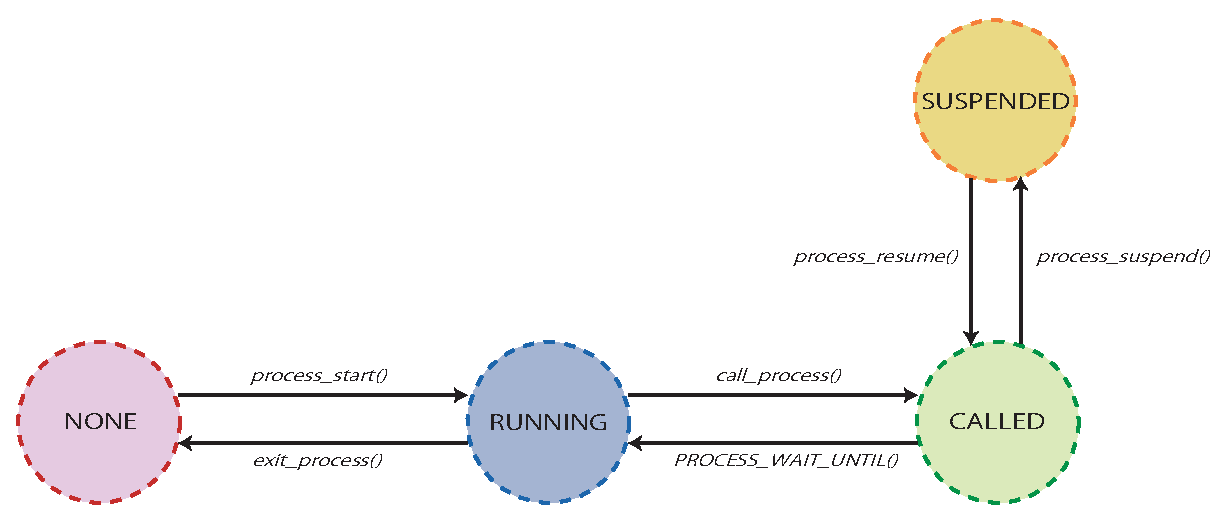
\includegraphics[width=130mm]{./images/state_transition.eps}
 \end{center}
 \caption{状態遷移図}
 \label{fig:state_transition}
\end{figure}


\section{まとめ}
本章では,
最初に本システムに必要な要件についてまとめ,
システムの概要について述べた.
そして,システムアーキテクチャを各モジュールに分解しながら説明し,
システム構成について考察した.
最後に実装環境など実装に関する内容について言及した.



%本章では,まず,ソフトウェアの構成について述べた,そして,個々のモジュールの細かな設計と実装について述べた.特に重要なアルゴリズムについては,各小節の末尾に実際のプログラムを掲載した.
